\chapter{Visual Design}

Visualizing syntenic data is a multi-faceted problem as not only can the visual representation change based on the underlying biological question but also the resolution at which the information is being visualized. In designing a solution for this problem, the taxonomy of design space created by previous synteny visualizers like Mizbee \cite{Meyer2009} was adopted and further enhanced with our recommendations for representing synteny in multi-way comparisons. This taxonomy of design space is centred around using visual variables to highlight the location, size and orientation of the conserved regions. In designing SynVisio we used two primary forms of visual representations, a parallel plot and a dot plot, and modified them to work across multiple resolution levels. We also created hybrid plots based on our parallel plot design to represent synteny in multi-way comparisons. In this chapter, we first discuss the different forms of visual encoding used in our system. We follow this with a  description of the different layout strategies that were explored. Then we elaborate on the various interaction strategies we adopted based on the visual information seeking mantra framework and design of multiple coordinated views. Finally we end the chapter with a discussion on our iterative design process through four major development cycles.

\begin{figure}[h]
  \centering
  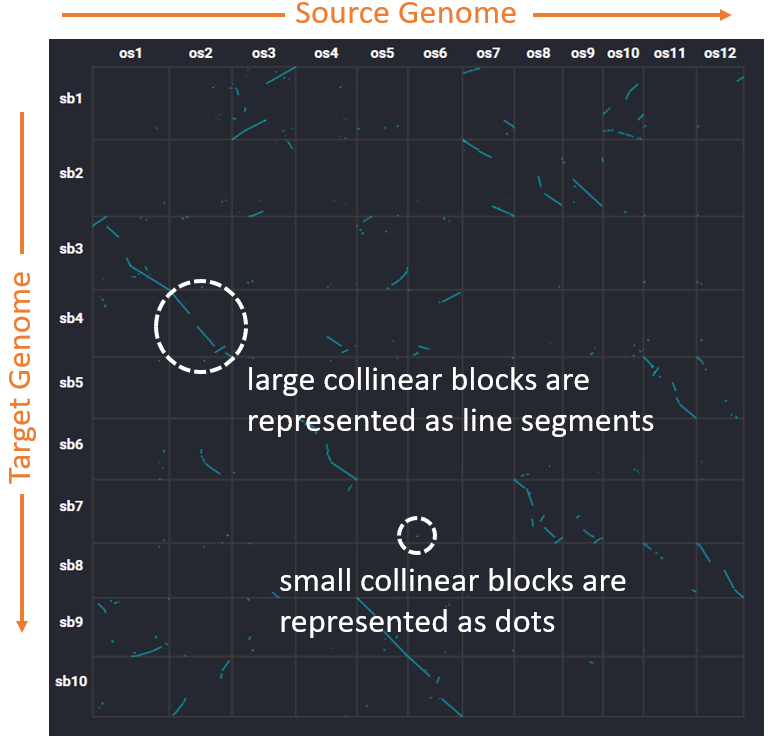
\includegraphics[width=.475\linewidth]{images/ch_4_dot_plot_a.PNG}
  \captionof{figure}{Dot plot showing whole genome synteny between Rice \textit{(Oriza sativa)} and Corn \textit{(Sorghum bicolor)} with grid-lines added for chromosomal boundaries.}
  \label{fig:ch_4_dot_plot_a}
\end{figure}


\section{Visual Encoding}

A common way to represent sequence alignment or similarity is to visualize it as a two-dimensional `dot plot' \cite{SONNHAMMER1995GC1,Cabanettes2018} through positional encoding. We adopted this strategy for our first visual representation by placing the source and target genomes along the \textit{x} and \textit{y} axes, respectively, and marking gene alignments with dots as shown in Figure \ref{fig:ch_4_dot_plot_a}. Grid-lines were then further added to the plot to indicate chromosomal boundaries.



This plot can also be adopted for other resolutions by changing the genomes along \textit{x,y} axes to either individual chromosomes or smaller gene blocks. Such matrix-based representations are very good at providing an overview of the dataset and can be used to highlight breaks, inversions, and duplications, as shown in Figure \ref{fig:ch_4_dot_plot_b}. However, being a relatively primitive visual representation dot plots are often found to be visually unappealing and complex to understand without the proper background context, making them unsuitable for a variety of exploration and communication tasks.


\begin{figure}
  \centering
  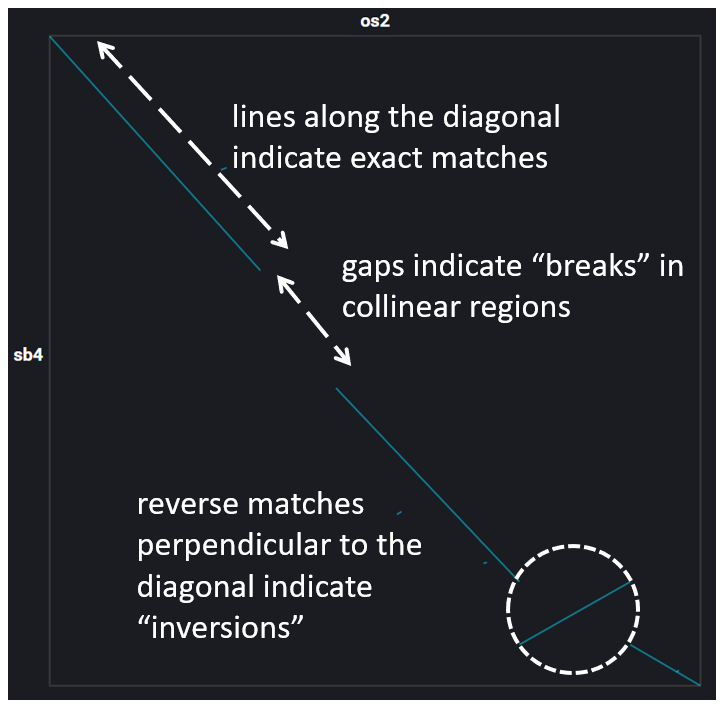
\includegraphics[width=.475\linewidth]{images/ch_4_dot_plot_b.PNG}
  \captionof{figure}{Dot plot showing breaks, inversions and duplication events between chromosome 2 and 4 of Rice \textit{(Oriza sativa)} and Corn \textit{(Sorghum bicolor)} respectively.}
  \label{fig:ch_4_dot_plot_b}
\end{figure}


For our other primary visual representation, we adopt a design that represents synteny through a combination of positional encoding for genomic distances and connected lines for similarity. In this approach, genomic sequences are stacked horizontally parallel to each other, and similar genes are connected through lines to indicate similarity. However, unlike dot plots that use the same visual encoding across all genomic sizes, for this visual representation, we adopt a different secondary encoding based on the resolution of the genomic sequences being visualized. 

\begin{figure}
  \centering
  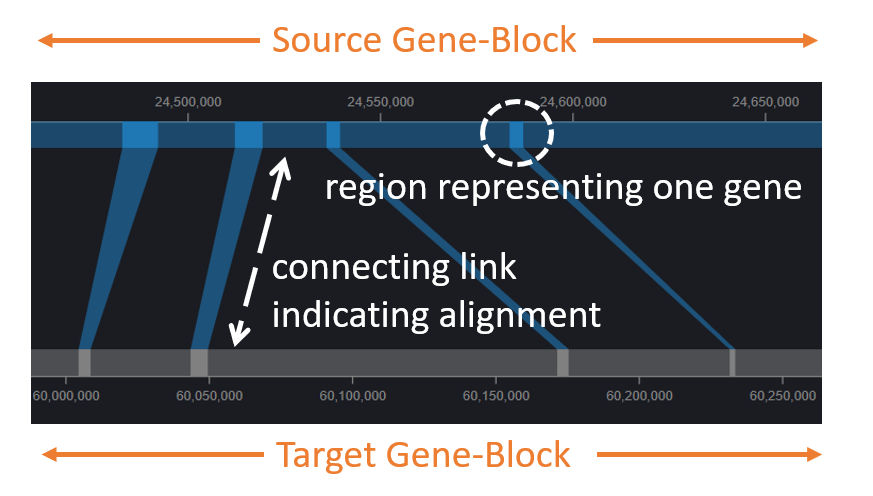
\includegraphics[width=.50\linewidth]{images/ch_4_link_plot.PNG}
  \captionof{figure}{Parallel plot at the gene-block level}
  \label{fig:ch_4_link_plot}
\end{figure}


There are three basic levels in which synteny can be visualized starting from the gene block level, which is the smallest unit at which syntenic data is reported. A gene block is a collection of collinear genes in the source genome that are aligned to a group of collinear genes in the target genome. To encode conservation at this level, we use two gene blocks that are represented by line segments, and are stacked parallel to each other. Similar genes within the blocks are then connected with ribbons, as shown in Figure \ref{fig:ch_4_link_plot}. The connecting ribbons are four sided polygons whose edge widths are dependent on the number of gene pairs in the collinear block at each edge. The source and target gene blocks are annotated with numeric tracks corresponding to their position in the chromosome and are coloured in distinct colours to distinguish them. The individual genes are represented as rectangles highlighted with a deeper shade of the base colour of the track for easier reference. 

At the next level, individual chromosomes are considered since a collection of gene blocks form a chromosome. Visualizing synteny at this level involves encoding information related to the location, size and orientation of conserved regions. To achieve this, chromosomes are stacked parallel to each other and their lengths are encoded to reflect their genomic size. So chromosomes with more base-pairs in them show up as wider line segments. Conserved regions in the chromosomes are then connected through ribbons from their positions on the chromosome to indicate similarity. This encodes both the location and the size of the conserved regions as the width of ribbons changes based on the genomic size of the linked gene blocks.


\begin{figure}[h]
  \centering
  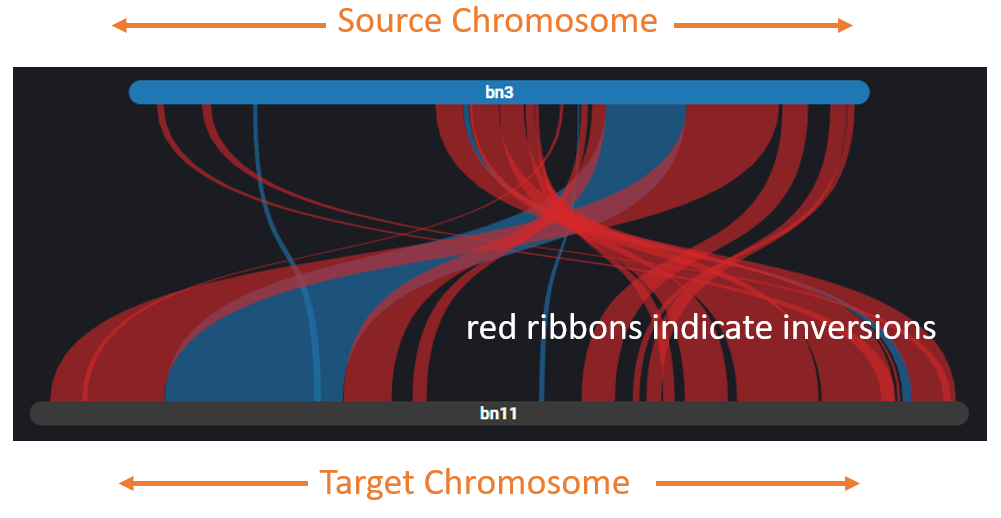
\includegraphics[width=.60\linewidth]{images/ch_4_link_plot_chromosome_a.PNG}
  \captionof{figure}{Link Plot at the Chromosome level where the blue coloured ribbons represent forward matches and the red coloured ribbons represent reverse matches (inversions).}
  \label{fig:ch_4_link_plot_chromosome_a}
\end{figure}


To encode the orientation of the gene block, secondary encoding in the form of colour is adopted to visually distinguish gene inversions, as shown in figure \ref{fig:ch_4_link_plot_chromosome_a}. So forward matches are coloured in blue, and reverse matches are coloured in red. Unlike the gene block level, at the chromosome level several bands can overlap and cross each other due to multiple gene translocation and inversions events and can cause visual clutter. To mitigate this problem, complex polygons are used instead of rectangular ribbons and are generated through \textbf{B}-spline curves\cite{ref851370272} with control points set to bundle the curves towards the centre\cite{zhou2013edge}. The control points are adjusted to be vertically in the middle of the parallel blocks to ensure that the original size of the ribbons remain undistorted at regions where they join the chromosome as they visually represent the size of the conserved region as shown in figure \ref{fig:ch_4_link_plot_chromosome_b}. 

\begin{figure}
  \centering
  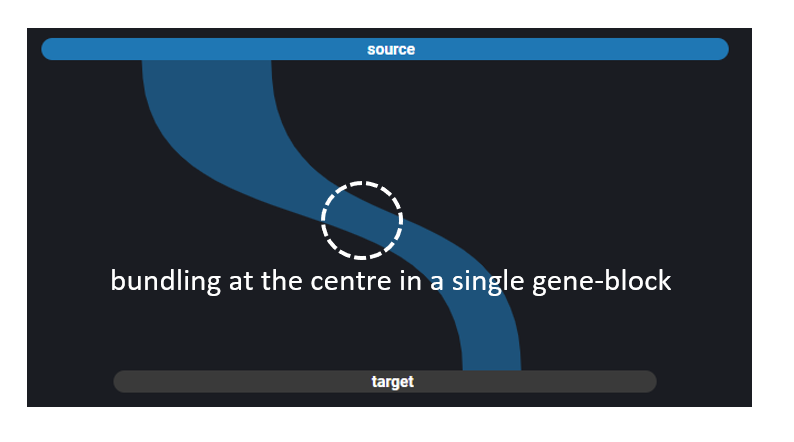
\includegraphics[width=.50\linewidth]{images/ch_4_link_plot_chromosome_b.PNG}
  \captionof{figure}{Ribbon bundling to reduce visual clutter with the control points set towards the centre indicated in a single gene-block.}
  \label{fig:ch_4_link_plot_chromosome_b}
\end{figure}


Finally, at the whole genome level where synteny is observed between several chromosomes at once, the chromosomal source of the collinear regions is given higher priority, and so secondary encoding in the form of colour is used to distinguish different chromosomes. A layout similar to the parallel stacking at chromosome level is adopted, however, instead of having a single connected unit for the entire genome, chromosomes are separated from each other with gaps serving to indicate the start and end of each chromosome. Chromosomes in the source layer are assigned a unique colour, while chromosomes in the target layer are assigned colours through an alternating gray and black colouring scheme. Ribbons are then linked between conserved regions to represent syntenic gene-blocks and are assigned a colour based on their source chromosome. This form of encoding location information about the source in the connection through colour has been used earlier in other synteny visualisation systems and has been proved effective \cite{Meyer2009}. We adopt the aforementioned bundling strategy of using \textbf{B}-spline curves\cite{ref851370272} to improve visual clarity but set the control points independently for every chromosome to group all the gene blocks emerging from each chromosome into a single bundle. Finally, inverted regions at this level are represented through ribbons that are wide at the extremities and pinched to be only a pixel wide at the centre which gives the visual impression of a flipped ribbon.


\begin{figure}[ht]
  \centering
  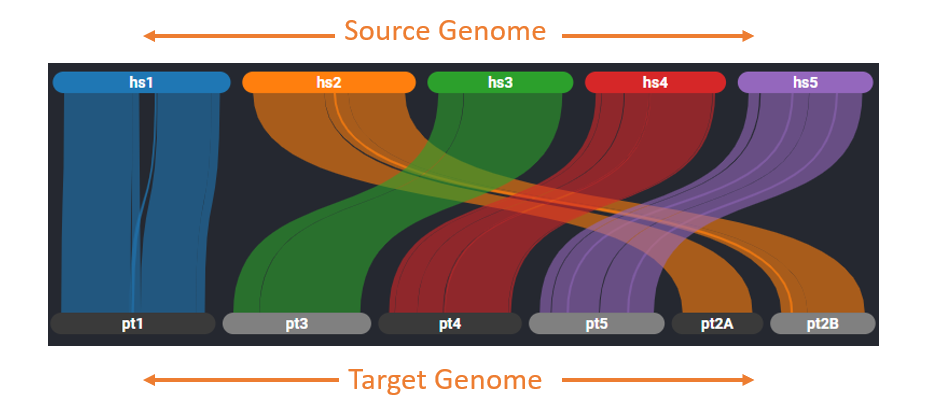
\includegraphics[width=.75\linewidth]{images/ch_4_genome_level.PNG}
  \captionof{figure}{Visual encoding at the chromosome level with connecting ribbons coloured based on the source chromosome they are linked from.}
  \label{fig:ch_4_genome_level}
\end{figure}



\section{Layout Strategies}

A common strategy that is used among all the three parallel stacked representations is the vertical separation between the source and the target to visually distinguish the two regions. This is easy to implement at the gene-block level, and the chromosome level as the source and target regions are single continuous entities but requires minor adaptations at the genome level. The genome is a combination of several chromosomes, so each chromosome had to be individually distinguishable while still being represented as a part of the whole source group and different from the target group. To achieve this grouping, we use the visual law of proximity from Gestalt principles \cite{wertheimer1923untersuchungen} which states that proximity can override other visual similarities (shape, size, colour) to differentiate a group of objects. and represent each chromosome as a pill-shaped region and then lay them out end to end horizontally with small gaps between them. The gaps between the chromosomes achieve the task of making the chromosomes look distinct and also being smaller than vertical gaps between the two genomes, clustering the source and the target regions into two separate groups visually.

\begin{figure}
  \centering
  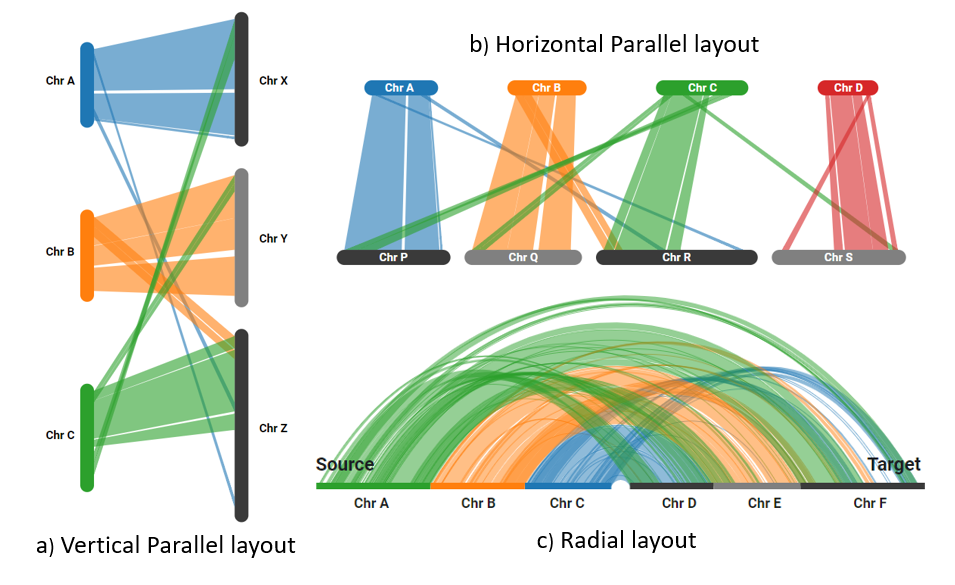
\includegraphics[width=.85\linewidth]{images/ch_4_layout.PNG}
  \captionof{figure}{Different layout strategies at the genome level with conservation being encoded as connections.}
  \label{fig:ch_4_layout}
\end{figure}


In arriving at the optimal layout strategy, we looked at several different alternative ways of arranging the chromosomes. In the popular synteny browser MizBee\cite{Meyer2009} the authors provide a taxonomy of the different synteny layouts and broadly classify them into two categories: contiguous and discrete. In the former, the chromosomes are presented adjacent to each other either in a linear or a circular layout, and in the later, chromosomes are treated as distinct elements, and presented either in segregated groups or interleaved with each other. In our design we go for the contiguous scheme, but we omit the circular layout as it has already been explored in AccuSyn\cite{accusyn}  and instead look at possible linear layout strategies where conservation is encoded through connections as shown in Figure \ref{fig:ch_4_layout}. In the vertical (a) and horizontal layouts (b) the underlying approach is similar except for the orientation of the two parallel layers. However the number of chromosomes in a genome can be numerous as in the case of humans who have 23 and can cause the vertical layout to be quite long. This makes it sub-optimal for the horizontal ``landscape'' aspect ratio of most computer monitors. Therefore of the two, the horizontal parallel layout is the preferred mode of encoding synteny. A common advantage of these two layouts is that they can be stacked in multiple layers such that chromosomes at every level are linked to both chromosomes above them and also the chromosomes below them, as shown in the layout (a) in Figure \ref{fig:ch_4_layout_multi}. This stacked layout strategy is used to represent synteny in the form of a tree view chart and can be particularly useful in scenarios where conserved regions need to be traced across several evolutionary levels.

\begin{figure}[ht]
  \centering
  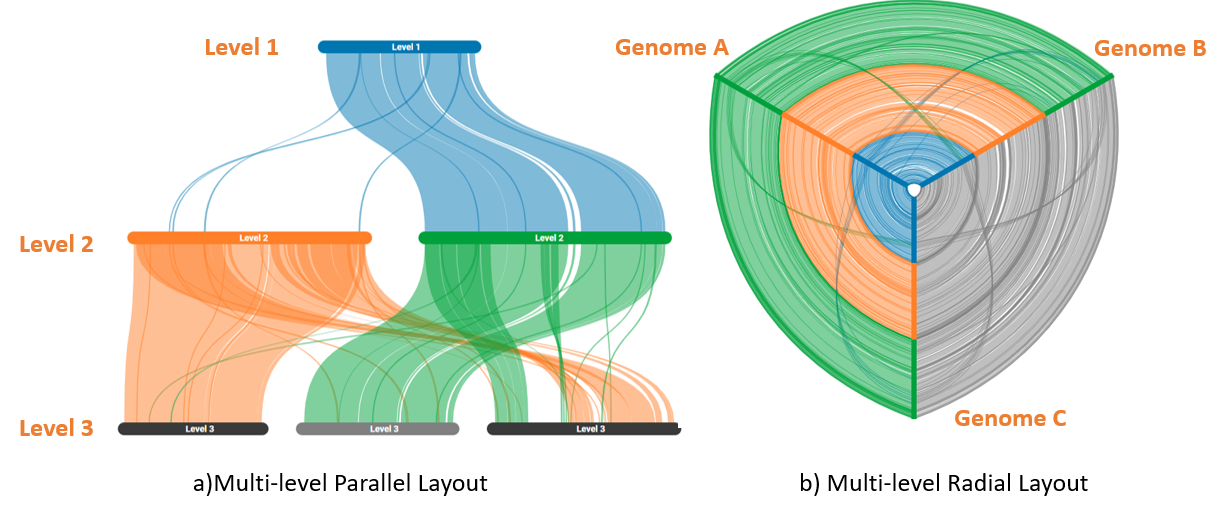
\includegraphics[width=.95\linewidth]{images/ch_4_layout_multi.PNG}
  \captionof{figure}{Multi-level layouts: Parallel layout (left) and Radial layout (right).}
  \label{fig:ch_4_layout_multi}
\end{figure}

The bi-directional linking strategy is however, unavailable in the parallel layout scheme in pairwise comparison scenarios but can be utilized by moving the two layers adjacent to each other, as shown by the layout (c) in Figure \ref{fig:ch_4_layout}. In this layout,  the chromosomes are in the same level, making it possible for conserved regions to be linked in two directions either from the top or from below. This allows us to include an additional layer of encoding. For example, if we had to represent the orientation of the conserved regions, we could link all forward matches through connections from the top, and all reverse matches through links from the bottom. The disadvantage of this layout is the high number of crossing between the connections. This can be made worse in scenarios where there is a high degree of collinearity between the two genomes due to the ordering of the chromosomes as every connection between the first chromosome in the source and the first chromosome in the target is crossed by all other connections emerging from the rest of the chromosomes in the source. An alternative approach to solve this problem includes reversing the layout of one of the layers or arranging the chromosomes in a radially outwards fashion in both the layers. This layout can also be extended to express synteny in multiple levels by merely increasing the number of radial layers such that each layer is connected to both the layer on its right and the layer on its left, as shown in the layout (b) in Figure \ref{fig:ch_4_layout_multi}.



Irrespective of the ordering or the layout of the chromosomes, they all have unique positions in a visual representation. This prevents them from being occluded by other items in that representation. This however is not the case for  visual encoding of conservation through lines or ribbons that can overlap significantly in some instances. The Z-axis position of the ribbons (i.e., the stacking order in the view) decides which ribbons occlude others and is dependent on the rendering order of the ribbons. To address this problem, we sort the conserved genes in every chromosome based on their gene count. This places smaller gene blocks at the end of the list ensuring that these blocks are rendered last, making them appear higher on the Z-axis and thus above the bigger blocks. To further solve this problem, connected ribbons are rendered with 75\% transparency, which ensures that even if ribbons end up overlaying other connected ribbons, they are still visible on the screen.

\section{Visual and Interaction Design}

Having discussed the different ways in which syntenic data can be encoded, we can summarise that the usefulness of a particular representation depends on the syntenic relationship under investigation. This has created a need for an adaptive system that can be used under a wide range of scenarios spanning investigation of micro synteny all the way up to high-level genome duplication events. Syntenic data also goes beyond the basic location, size and orientation of the conserved regions and includes additional information such as the match score and the E (expect) value, which indicates the level of similarity and the probability of a match occurring by chance. This inherent complexity in the dataset means that exploring it becomes challenging as the volume of the data increases. Thus in designing our synteny exploration interface, we build on the framework of ``visual information seeking mantra'', which offers standard visual design guidelines for developing information visualization applications \cite{Shneiderman96theeyes}. The framework can be used to break down synteny analysis broadly into the following tasks: overview, filter, zoom, details-on-demand, history, and extract.

We present information in a top-down tiered approach in three distinct scales starting with the whole genome followed by stepping down into an individual chromosome and finally ending on the gene block level. Users are given the ability to start their investigation of the data at any particular level and pick either a dot plot, or a parallel plot, or a combination of both. Users are then given the option to interact with the visualizations in real-time to either filter the chart to look at conserved regions in a particular chromosome or drill down into the dataset all the way down to an individual gene in a conserved region as shown in Figure \ref{fig:ch_4_exploration_through_interaction}. Additional details about the syntenic blocks are available on-demand through hover-based mouse interactions either with the ribbons or the dots based on the type of representation.

\begin{figure}[h]
  \centering
  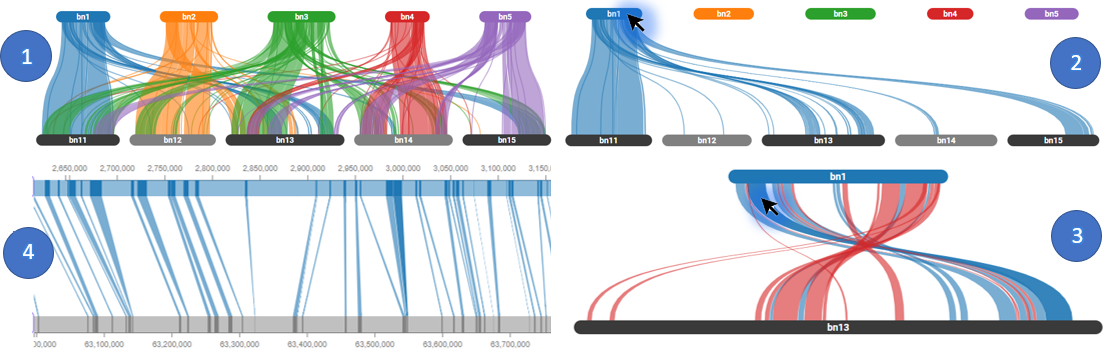
\includegraphics[width=1\linewidth]{images/ch_4_exploration_through_interaction.PNG}
  \captionof{figure}{User interactions in exploring conserved regions in a top down approach through four steps pictured in clockwise fashion.}
  \label{fig:ch_4_exploration_through_interaction}
\end{figure}


Our design also incorporates a dashboard for exploration where instead of relying on a single visualization, information about conservation at every level is presented through coordinated multiple views. This is built on the underlying premise that users have a better understanding of their data if they interact with the given information and view it through different representations\cite{Roberts}. In our design of multiple distinct views that support the investigation of a single entity, we followed the design guidelines set by earlier research into multiple coordinated views in information visualization systems\cite{WangBaldonado}. We present the following three distinct views, each highlighting a unique facet of the dataset: parallel plot, dot plot and a simple scatter plot that acts as a filter toggle. The parallel plot offers position and location information about the conserved regions at a glance while the dot matrix plot can easily highlight reversals and deletions within the conserved regions. Both the views are linked to each other to ensure that users don't lose context of their interaction. This is done by mirroring all actions between the two views. The final scatter plot is used to present the measure of similarity of the conserved regions and has a slider built into it that can be used to filter conserved regions based on their match score or E value. The filter works synchronously with the other two views and as the user moves the slider, the conserved regions are filtered in real time in the other two views. Finally, in keeping with the visual information seeking mantra framework, user interactions are recorded with users having the ability to store all their interactions in arriving at a particular analysis point as a visual stamp that can be revisited or reset back to in-case of further analysis.

\section{Iterative Development Process}
By following the guidelines of a standard design study methodology\cite{5290695}, our system design occurred iteratively over four main development cycles. At every stage, we presented our system to a panel composed of genome researchers and information visualization experts to gather feedback and look at possible avenues of improvement. After the initial requirement gathering phase we sketched a prototype of a linear parallel plot and a dot plot both visualizing conserved regions at the genome level. For our first development cycle, we used basic colours for distinguishing different chromosomes and encoded every collinear gene as a connecting link in the parallel plot and as a single point in the dot plot, as shown in Figure \ref{fig:ch_4_first_iteration}. Although this approach helped in highlighting large scale patterns in genomic conservation, encoding every single gene meant that there was significant noise in the visualization that made it difficult to see the smaller conserved regions. Feedback was also directed at the choice of colour and and the layout of the lines in the parallel plot that caused them to visually occlude the lines right below them.

\begin{figure}
  \centering
  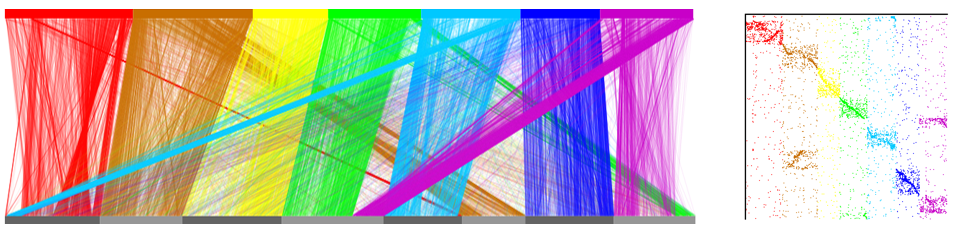
\includegraphics[width=1\linewidth]{images/ch_4_first_iteration.PNG}
  \captionof{figure}{Visual representations after the first development cycle consisting of a parallel plot (left) and a dot plot (right).}
  \label{fig:ch_4_first_iteration}
\end{figure}

\begin{figure}[h]
  \centering
  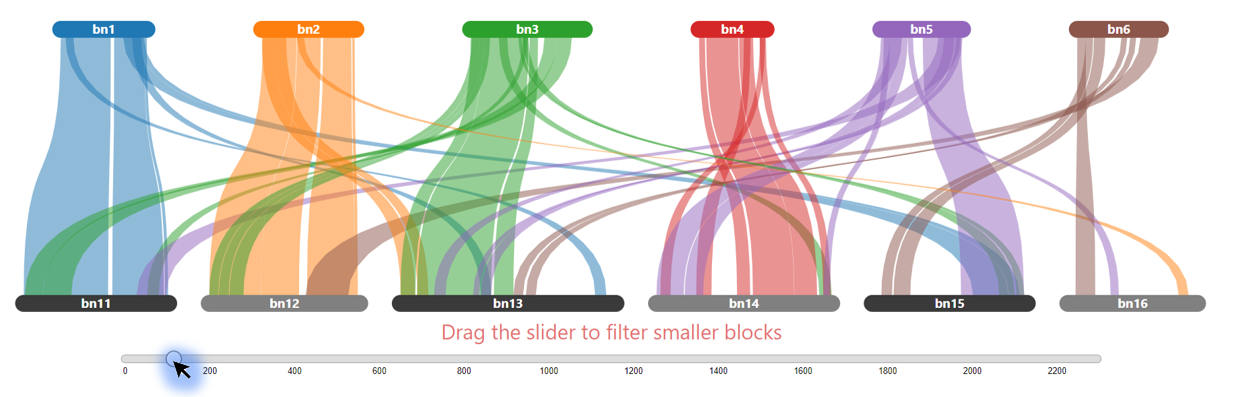
\includegraphics[width=0.85\linewidth]{images/ch_4_base_viewer.PNG}
  \captionof{figure}{Design after the second development cycle with a slider filter.}
  \label{fig:ch_4_base_viewer}
\end{figure}


For our second development cycle, we adopted two major changes: we divided the syntenic data into three levels and limited top level visualizations to just representing collinear gene blocks instead of their constituent genes and, we added interaction features that let users select the chromosomes they wanted to observe instead of looking at the entire genome. Although grouping collinear genes into larger blocks helped reduce visual occlusion, this problem was further addressed by an updated colour palette and converting connecting ribbons into curved B-spline ribbons instead of straight rectangular strips. Since dot plots are based on positional encoding we removed colours to identify chromosomes in the dot plots and instead relied on grid lines to act as chromosomal boundaries. New levels at the chromosome and the gene-block level were also added to visualize conservation at smaller scales. Finally, a simple slider interface was added to filter conserved blocks based on their gene count. Feedback at this level was largely directed towards the filter feature which despite being helpful was counter-intuitive to synteny exploration as the relevance of conserved regions is based on a combination of the level of similarity , the probability of the match occurring by chance and its constituent genes and not just the gene count. This is because filtering conserved regions is highly dependent on the subject under exploration and hence it needs to be contextually adaptive.


Development in our third iteration was structured around building a system that could be adapted for use in a wide range of scenarios. We developed a composite dashboard with coordinated views and a context-aware filter to help users in making a better-informed decision when they are filtering syntenic blocks. To improve usability, we also added multi-level comparison charts such as hive plots and stacked parallel plots to represent synteny beyond simple pairwise scenarios. For our fourth and final development iteration, we added features that were designed to improve user engagement with our interface, such as gene search and addition of secondary visual encoding in the form of heat-map or histogram tracks to the chart. Visual encoding for the gene search feature was primarily done through colour and vertical positioning. A gene block that contained the gene being searched for was coloured in white and brought to the front above the other gene blocks in terms of on-screen rendering in order to highlight it.